\chapter{Resultados y Discusi\'on}

Durante la ejecuci\'on del algoritmo se realizaron m\'ultiples corridas completas para cada funci\'on objetivo (Langermann y Drop-Wave), lo que permiti\'o evaluar la estabilidad y eficiencia del m\'etodo. Los resultados se agruparon en res\'umenes globales\footnote{Se anexan tablas de los resumenes independientes de cada ejecución en la seccion de resumenes e historiales correspondiente a cada función dentro del capitulo de anexos.}, donde se registraron indicadores clave, los cuales sencuentran dentro de la siguientes tablas:
\begin{longtable}{lrrr}
\caption{Archivo: resumen\_global\_corridas\_langerman}\label{tab:resumen_global_corridas} \\
\toprule
Indicador & x1 & x2 & Fitness \\
\midrule
\endfirsthead
\toprule
Indicador & x1 & x2 & Fitness \\
\midrule
\endhead
\midrule
\multicolumn{4}{r}{Continued on next page} \\
\midrule
\endfoot
\bottomrule
\endlastfoot
Mejor (Fitness) & 2.002592498731848 & 1.006380979616417 & -5.162121824564412 \\
Peor (Fitness) & 2.095881924190502 & 0.7727067906304386 & -4.914015915528873 \\
Media & 2.0147728529858315 & 0.9775829446121328 & -5.13507342254136 \\
Desv. Estándar & 0.0275004061456432 & 0.0688284607116998 & 0.0738337377292753 \\
\end{longtable}
\begin{longtable}{lrrr}
\caption{Archivo: resumen\_global\_corridas\_langerman}\label{tab:resumen_global_corridas} \\
\toprule
Indicador & x1 & x2 & Fitness \\
\midrule
\endfirsthead
\toprule
Indicador & x1 & x2 & Fitness \\
\midrule
\endhead
\midrule
\multicolumn{4}{r}{Continued on next page} \\
\midrule
\endfoot
\bottomrule
\endlastfoot
Mejor (Fitness) & 2.002592498731848 & 1.006380979616417 & -5.162121824564412 \\
Peor (Fitness) & 2.095881924190502 & 0.7727067906304386 & -4.914015915528873 \\
Media & 2.0147728529858315 & 0.9775829446121328 & -5.13507342254136 \\
Desv. Estándar & 0.0275004061456432 & 0.0688284607116998 & 0.0738337377292753 \\
\end{longtable}

Donde cada Indicador Representa lo siguiente:
\begin{itemize}
    \item \textbf{Mejor (Fitness):} Representa la soluci\'on con el valor de fitness m\'inimo obtenido en todas las corridas.
    \item \textbf{Peor (Fitness):} Indica la soluci\'on con el mayor valor de fitness, sirviendo como referencia de la variabilidad en la b\'usqueda.
    \item \textbf{Media:} Es el promedio de los valores de fitness de la mejor soluci\'on de cada corrida, ofreciendo una visi\'on global del desempe\~no del algoritmo.
    \item \textbf{Desv. Est\'andar:} Mide la dispersi\'on de los valores de fitness entre las corridas, reflejando la estabilidad y consistencia del proceso evolutivo.
\end{itemize}

\section{An\'alisis de los Resultados}

\subsection{Consistencia y Robustez}
Los res\'umenes globales muestran que, a lo largo de las corridas, el algoritmo tiende a converger de manera consistente hacia soluciones de alta calidad. Una baja desviaci\'on est\'andar en los valores de fitness sugiere que el proceso evolutivo es robusto y no depende en exceso de la aleatoriedad inherente a los operadores gen\'eticos. Esto es crucial para problemas de optimizaci\'on, ya que garantiza que la metodolog\'ia aplicada es reproducible y confiable.

\subsection{Comparaci\'on Entre Funciones}
\subsubsection{Funci\'on Langermann}
El resumen global para Langermann indica que el algoritmo fue capaz de identificar una soluci\'on cercana al \'optimo global, a pesar de la presencia de m\'ultiples \'optimos locales debido a la naturaleza multimodal de la funci\'on. El valor de ``Mejor (Fitness)'' obtenido se sit\'ua en un rango competitivo, y la media de las corridas respalda la eficacia del operador SBX y la mutaci\'on polinomial para explorar el espacio de soluciones.

\subsubsection{Funci\'on Drop-Wave}
Para la funci\'on Drop-Wave, que presenta una superficie de b\'usqueda ondulada, los resultados globales evidencian una convergencia hacia regiones con valores de fitness bajos, a pesar de la complejidad inherente a la topolog\'ia de la funci\'on. Los indicadores de ``Peor (Fitness)'' y ``Desv. Est\'andar'' muestran que, aunque existen ciertas variaciones entre corridas, el mecanismo de elitismo y la correcta aplicaci\'on de los operadores gen\'eticos ayudan a mitigar posibles desviaciones, logrando resultados consistentes.

\subsection{Evoluci\'on del Fitness y Visualizaciones}
Las gr\'aficas de la evoluci\'on del fitness, tanto en su forma original como normalizada, permiten observar el progreso generacional. Se aprecia una clara tendencia a la mejora, donde la mayor\'ia de las corridas muestran una reducci\'on significativa del valor de fitness a medida que avanzan las generaciones.

A continuación se dejan las gráficas de la evolución del fitness:
\begin{figure}[H]
    \centering
    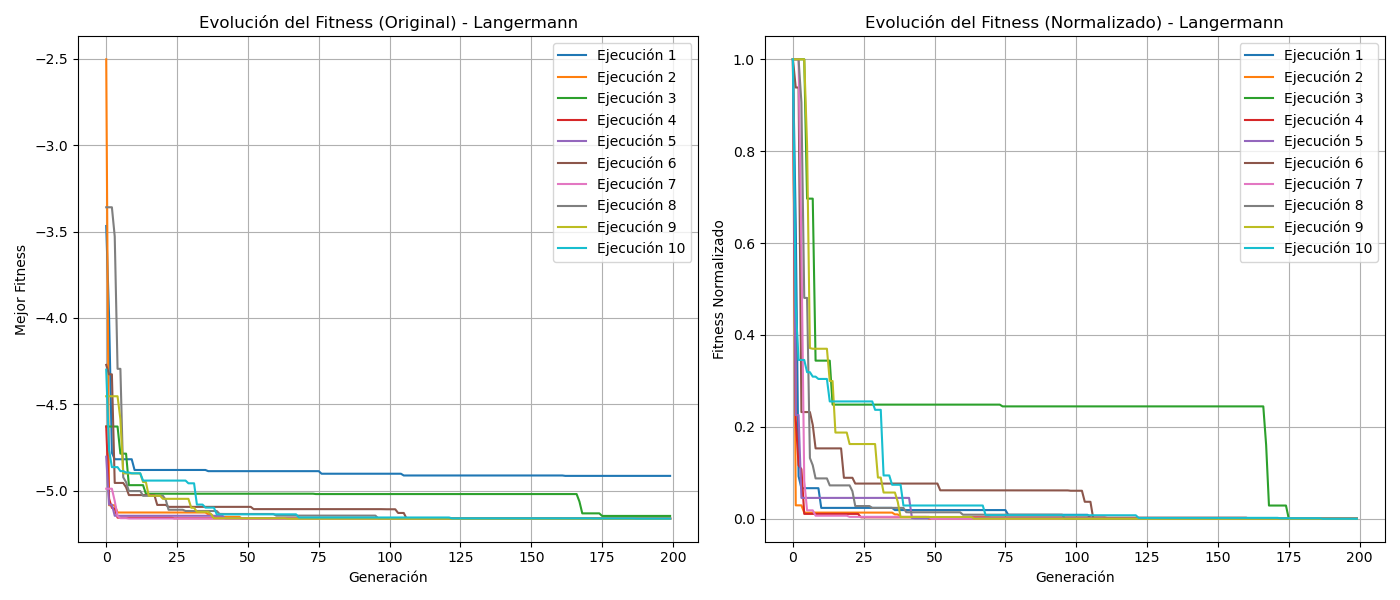
\includegraphics[width=\textwidth]{secciones/tablas/langermann/evolucion_fitness_langermann.png}
    \caption{Evolución del \text{fitness} de la función de Langermann}
    \label{fig:fitness_langermann}
\end{figure}

\begin{figure}[H]
    \centering
    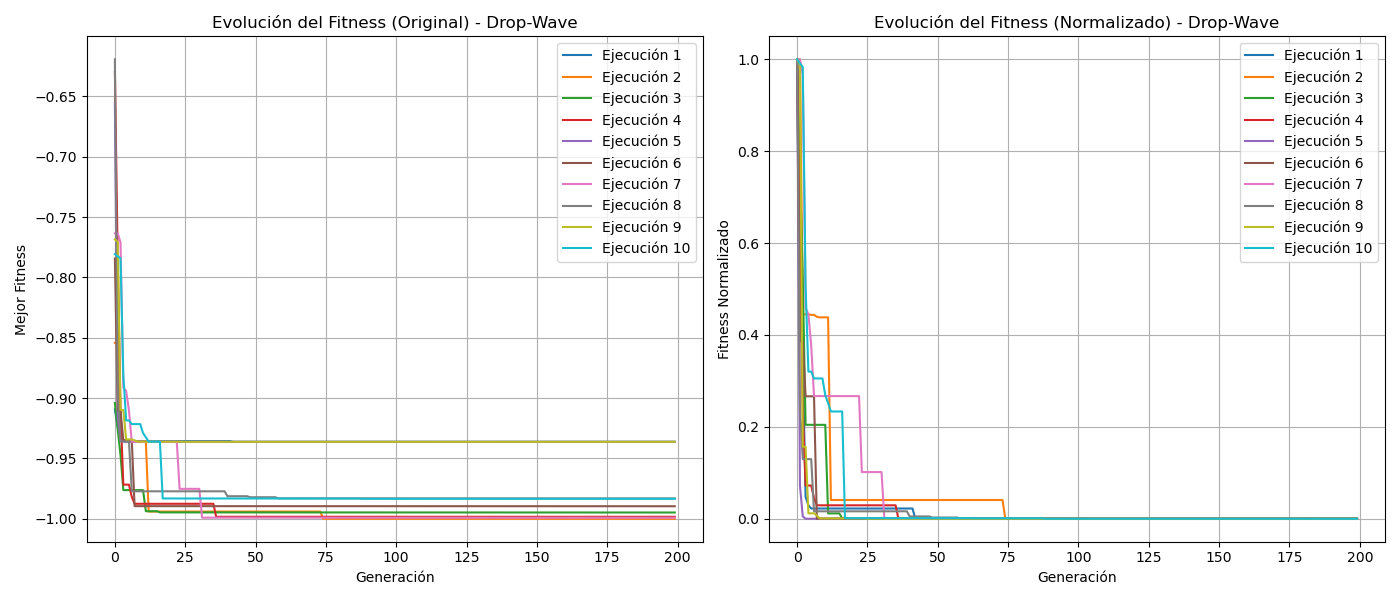
\includegraphics[width=\textwidth]{secciones/tablas/drop_wave/evolucion_fitness_drop_wave.png}
    \caption{Evolución del \text{fitness} de la función Drop Wave}
    \label{fig:fitness_drop_wave}
\end{figure}

Adem\'as, la visualizaci\'on 3D de la superficie de la funci\'on (para casos bidimensionales) complementa el an\'alisis, ya que permite ver la distribuci\'on espacial de las mejores soluciones encontradas en cada corrida. Esto confirma visualmente la capacidad del algoritmo para explorar eficazmente el espacio de b\'usqueda y concentrarse en las regiones prometedoras.

A continuación se dejan la visualización 3D de la superficie de las funciones y su proyección en el plano de las variables optimizadas:
\begin{figure}[H]
    \centering
    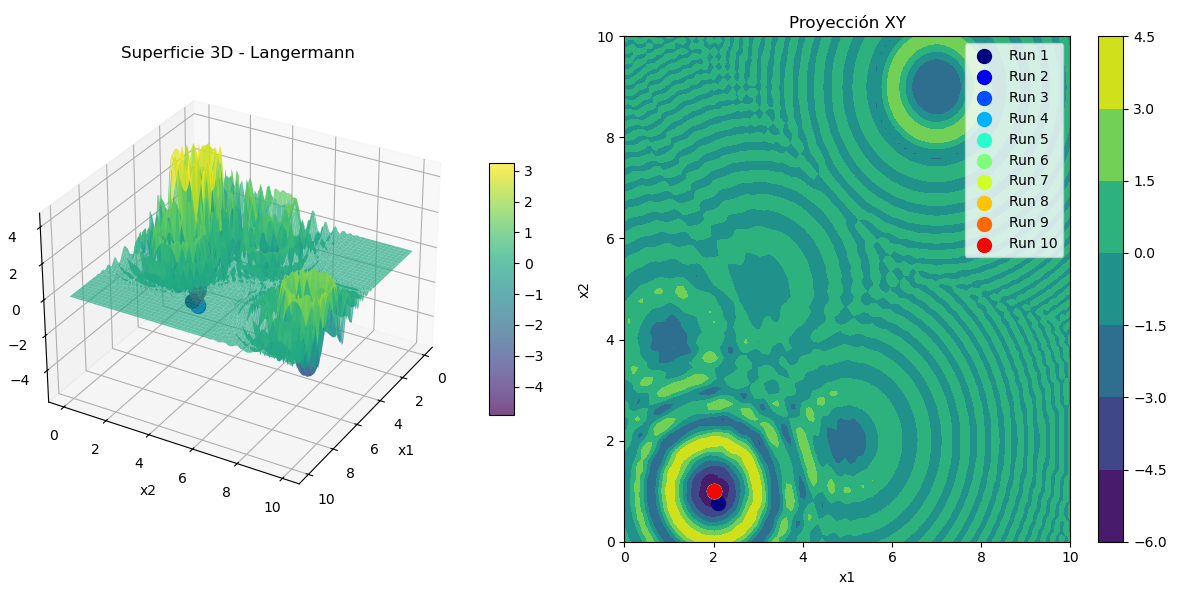
\includegraphics[width=\textwidth]{secciones/tablas/langermann/surface_3d_langermann.png}
    \caption{Representación y superficie de la función de Langermann}
    \label{fig:surface_langermann}
\end{figure}

\begin{figure}[H]
    \centering
    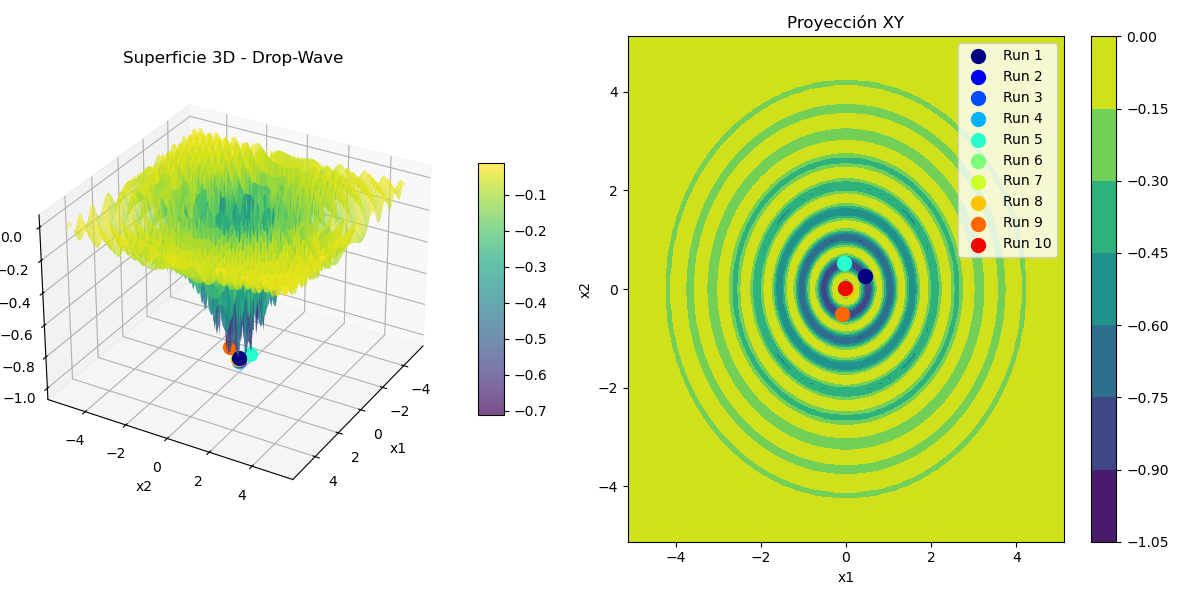
\includegraphics[width=\textwidth]{secciones/tablas/drop_wave/surface_3d_drop_wave.png}
    \caption{Representación y superficie de la función Drop Wave}
    \label{fig:surface_drop_wave}
\end{figure}

\section{Discusión Resultados}

\begin{itemize}
    \item \textbf{Eficacia del Algoritmo:} Los indicadores globales extra\'idos de los CSV demuestran que el algoritmo gen\'etico es capaz de acercarse a la soluci\'on \'optima, manteniendo una evoluci\'on progresiva y consistente en la reducci\'on del valor de fitness.
    
    \item \textbf{Diversidad y Convergencia:} La aplicaci\'on de operadores de selecci\'on, cruzamiento y mutaci\'on, junto con el mecanismo de elitismo, garantiza un equilibrio entre la exploraci\'on y la explotaci\'on del espacio de b\'usqueda. Esto se refleja en la baja variabilidad entre corridas, lo que es un indicativo de la estabilidad del proceso.
    
    \item \textbf{Potencial de Adaptaci\'on:} La estructura modular y la robustez mostrada por los resultados permiten considerar la posibilidad de aplicar este marco a otros problemas de optimizaci\'on, incluso aquellos con mayores dimensiones o con funciones objetivo de mayor complejidad.
\end{itemize}

